% Level ceiling (grade 6): density handled as "mass of one cubic
% centimetre" via proportionality tables and division; the literal
% formula rho = m/V waits for grade 7 (literal expressions, math g7).
\chapter{الكثافة: لماذا تطفو الأشياء}\label{ch:g6:density-floating}

في سنتك الأولى غرقت قطعة نقود صغيرة وطفا جذع عظيم، ووعدنا بأن
``اللماذا'' كنز من كنوز هذا المنهاج. وقد استحققته. فالمفتاح
صيغ عبر فصلين --- \omterm{def:g3:measuring-mass:mass}{الكتلة} للمادة، \omterm{def:g6:mass-and-volume:volume}{والحجم} للحيّز --- واليوم
يدوران معًا في القفل.

\section{كتلة سنتيمتر مكعّب واحد}

\begin{example}[مقارنة عادلة أخيرًا]\label{ex:g6:density-floating:fair}
لم تكن مقارنة جذع كامل بقطعة نقود كاملة عادلة قطّ: أحجام
مختلفة وأشكال مختلفة. أما المباراة العادلة فتأخذ \emph{أحجامًا
متساوية}: سنتيمترًا مكعّبًا واحدًا من كل متبارٍ. \omterm{def:g6:mass-and-volume:volume}{فسنتيمتر مكعّب}
من الماء كتلته \qty{1}{g}. \omterm{def:g6:mass-and-volume:volume}{وسنتيمتر مكعّب} من البلّوط: نحو
\qty{0.6}{g}. ومن الحجر: نحو \qty{2.5}{g}. ومن الحديد:
\qty{7.9}{g}. أحياز متساوية ومادة متفاوتة تفاوتًا جامحًا ---
وهذا هو العدد الذي كانت لعبة \omterm{def:g1:floating-and-sinking:words}{الطفو} تنتظره.
\end{example}

\begin{definition}[الكثافة]\label{def:g6:density-floating:density}
\emph{كثافة}\index{كثافة} مادة هي \omterm{def:g3:measuring-mass:mass}{كتلة} \omterm{def:g6:mass-and-volume:volume}{سنتيمتر مكعّب} واحد منها
بالغرامات. فكثافة الماء \qty{1}{g} لكل \unit{cm^3}؛ وكثافة
البلّوط نحو $0.6$؛ وكثافة الحديد $7.9$. ولإيجاد كثافة لا يلزم
جهاز جديد: قِس \omterm{def:g3:measuring-mass:mass}{كتلة} عيّنة وحجمها، ثم اقسم --- وزّع الغرامات
بالتساوي على السنتيمترات المكعّبة، فيكون الجواب حصة كل
\omterm{def:g2:measuring-length:units}{سنتيمتر}.
\end{definition}

\begin{omfigure}
\begin{tikzpicture}[scale=0.85]
  \foreach \x/\name/\m/\c in {0.9/فلّين/0.2/omMeth,
      3.0/بلّوط/0.6/omMeth, 5.1/ماء/1.0/omDef,
      7.2/حجر/2.5/omExo, 9.3/حديد/7.9/omThm} {
    \draw[thick, fill=\c, fill opacity=0.4]
      (\x,0.6) rectangle ++(1.0,1.0);
    \node[above, font=\footnotesize] at (\x+0.5,1.65) {\name};
    \node[below, font=\footnotesize] at (\x+0.5,0.5)
      {$\m$ g};
  }
  \node[below, font=\small] at (5.6,-0.15)
    {خمسة مكعّبات متساوية سعة سنتيمتر مكعّب --- وخمس كتل};
\end{tikzpicture}

{\small المباراة العادلة: الحيّز نفسه للجميع، فتُظهر كل مادة
كتلتها التي توقّعها.}
\end{omfigure}

\begin{proposition}[الكثافة توقيع]\label{prop:g6:density-floating:signature}
\omterm{def:g6:density-floating:density}{كثافة} مادة نقية واحدة في كل قطعة منها، كبيرة كانت أم صغيرة:
فشظيّة بلّوط وعارضة كاملة تحملان نحو \qty{0.6}{g} في كل
\omterm{def:g6:mass-and-volume:volume}{سنتيمتر مكعّب}. \omterm{def:g6:density-floating:density}{فالكثافة} إذن تعرّف الموادّ، كما تفعل درجات
\omterm{def:g6:water-states:changes}{الانصهار}: قِس \omterm{def:g3:measuring-mass:mass}{كتلة} جسم غامض وحجمه، واقسم، وقارن بالجدول ---
فكثيرًا ما تعترف المادة في الحال.
\end{proposition}

\begin{method}[كيف تقيس كثافة]\label{met:g6:density-floating:measure}
لحصاة --- أو لتاج:
\begin{enumerate}
  \item قِس كتلتها بالميزان: ولنقل \qty{75}{g}؛
  \item وقِس حجمها بارتفاع الماء: ولنقل \qty{30}{cm^3}؛
  \item واقسم الغرامات على السنتيمترات المكعّبة:
        $75 \div 30 = 2.5$ --- فكل \omterm{def:g6:mass-and-volume:volume}{سنتيمتر مكعّب} يحمل
        \qty{2.5}{g}؛
  \item وراجِع الجدول: \omterm{def:g6:density-floating:density}{الكثافة} $2.5$ --- فحصاتنا حجر عادي.
\end{enumerate}
\end{method}

\section{قاعدة الطفو}

\begin{proposition}[لماذا تطفو الأشياء]\label{prop:g6:density-floating:rule}
\omterm{def:g1:floating-and-sinking:words}{يطفو} الجسم في الماء إذا كانت كثافته \emph{أقلّ} من \omterm{def:g6:density-floating:density}{كثافة} الماء
--- أي أقلّ من \qty{1}{g} لكل \omterm{def:g6:mass-and-volume:volume}{سنتيمتر مكعّب} --- \omterm{def:g1:floating-and-sinking:words}{ويغرق} إذا كانت
كثافته أكبر. فالماء، إن صحّ التعبير، يقارن الداخل الجديد بنفسه،
حيّزًا بحيّز: فالأخفّ منّي لكل حيّز يركب في الأعلى؛ والأثقل لكل
حيّز ينزل. والقاعدة نفسها تحكم أي \omterm{def:g3:solids-liquids-gases:liquid}{سائل}، ولكل واحد كثافته حَكَمًا.
\end{proposition}

\begin{omfigure}
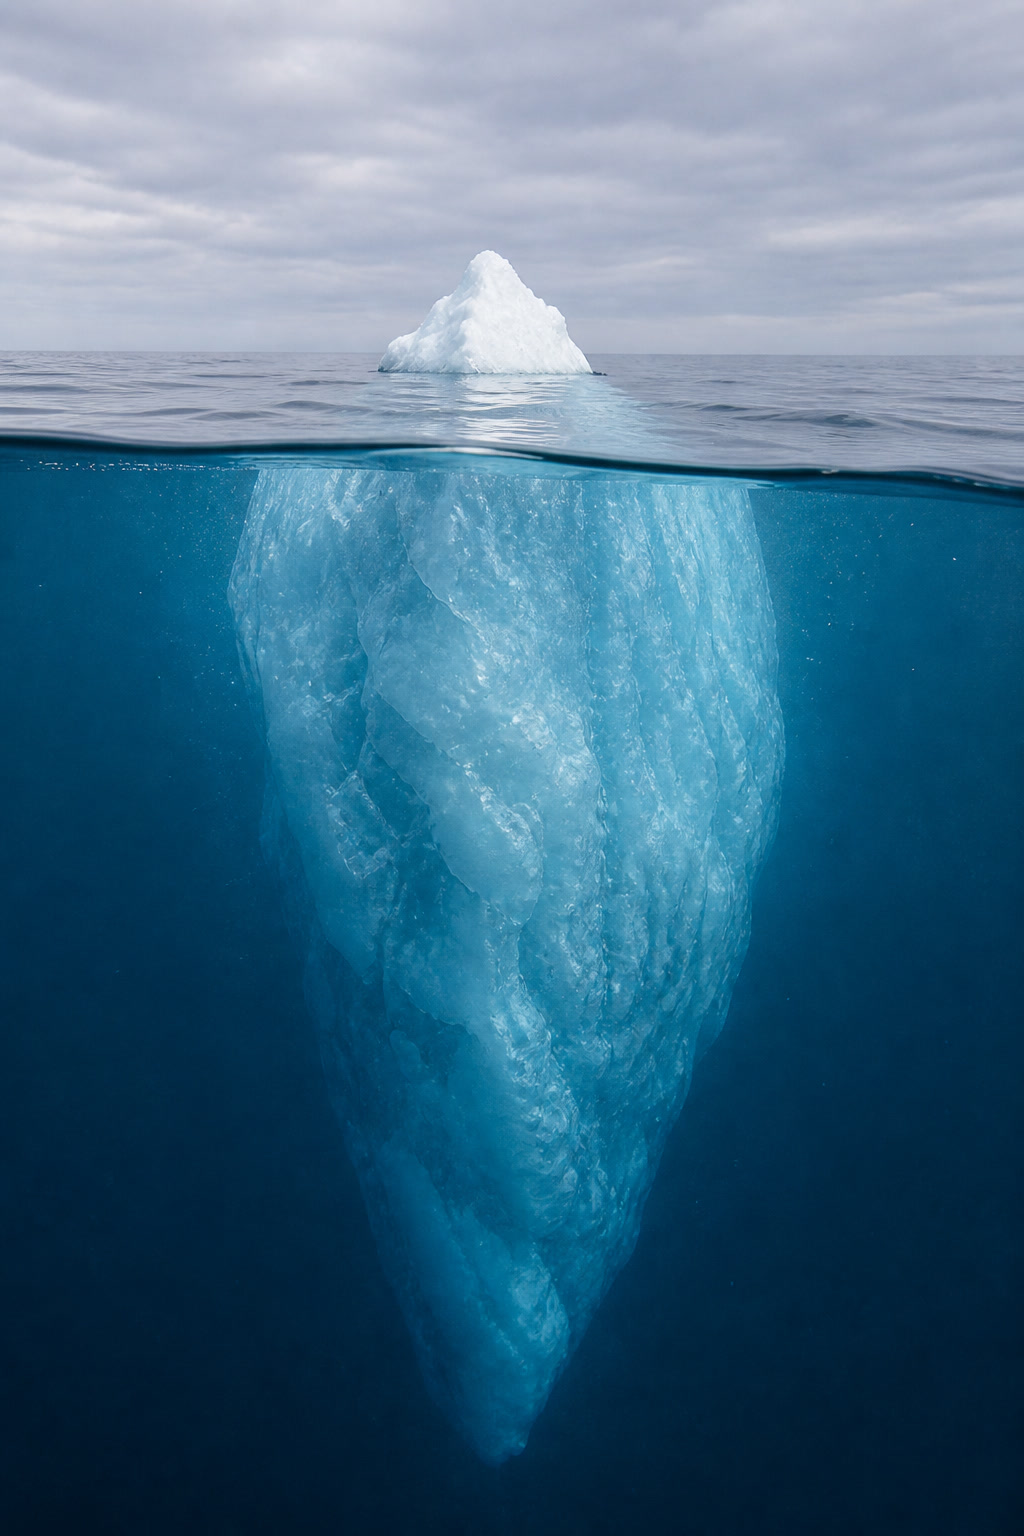
\includegraphics[width=0.4\linewidth]{images/book1/ai/g6-density-iceberg.jpg}

{\small الثلج أقلّ \omterm{def:g6:density-floating:density}{كثافة} من الماء بقليل لا غير --- \omterm{def:g1:floating-and-sinking:words}{فيطفو} الجبل الجليدي غاطسًا، مخبّئًا معظم كتلته تحت خطّ الماء.}
\end{omfigure}

\begin{example}[ستّ سنوات من الأحاجي، محسومةً]\label{ex:g6:density-floating:settled}
الجذع ($0.6$): \omterm{def:g1:floating-and-sinking:words}{يطفو}، مهما ضخم --- فكل \omterm{def:g6:mass-and-volume:volume}{سنتيمتر مكعّب} منه يزايد
دون الماء. وقطعة النقود (برونز، قرب $9$): تغرق، مهما صغرت.
والبطّة البلاستيكية والفلّينة والقلم: دون $1$، فكلها طافية.
والثلج، عند $0.9$ --- وهو صلب الماء المنتفخ --- \omterm{def:g1:floating-and-sinking:words}{يطفو} على سائله
بشعرة، ولهذا تلبس البِرَك أغطية وتبحر الجبال الجليدية. وقارب
المعجونة؟ مشكَّلًا وعاءً، يحمل طرد \emph{القارب مع \omterm{def:g2:air-around-us:air}{الهواء}}
هواءً كثيرًا لكل حيّز: فتهبط \omterm{def:g6:density-floating:density}{كثافة} الطرد دون $1$، وفي الموانئ
تُطلق الحيلة نفسها سفنًا فولاذية وزنها عشرة آلاف طنّ.
\end{example}

\begin{omfigure}
\begin{tikzpicture}[scale=0.85]
  \draw[thick] (0.8,0) -- (0.8,3.4) (4.0,0) -- (4.0,3.4)
    (0.8,0) -- (4.0,0);
  \fill[omMeth, opacity=0.35] (0.8,2.2) rectangle (4.0,3.0);
  \node[font=\footnotesize] at (2.4,2.6) {زيت: $0.9$};
  \fill[omDef, opacity=0.3] (0.8,1.1) rectangle (4.0,2.2);
  \node[font=\footnotesize] at (2.4,1.65) {ماء: $1.0$};
  \fill[omThm, opacity=0.3] (0.8,0.05) rectangle (4.0,1.1);
  \node[font=\footnotesize] at (2.4,0.55) {عسل: $1.4$};
  \node[below, font=\small] at (2.4,-0.3)
    {برج السوائل: الأكثف في القاع};
  \draw[thick] (7.2,0) -- (7.2,3.4) (11.0,0) -- (11.0,3.4)
    (7.2,0) -- (11.0,0);
  \fill[omDef, opacity=0.3] (7.2,0.05) rectangle (11.0,2.6);
  \draw[thick, fill=white]
    (8.3,2.35) -- (9.9,2.35) -- (9.6,2.95) -- (8.6,2.95) -- cycle;
  \draw[thick, fill=white, fill opacity=0.7]
    (8.0,2.35) -- (10.2,2.35) -- (9.5,1.0) -- (8.7,1.0) -- cycle;
  \node[font=\footnotesize] at (9.1,1.85) {ثلج: $0.9$};
  \node[below, font=\small] at (9.1,-0.3)
    {الجبل الجليدي: تسعة أعشاره تحت خطّ الماء};
\end{tikzpicture}

{\small خطّ \omterm{def:g6:density-floating:density}{الكثافة}: السوائل تتراصّ الأكثف في الأسفل، والثلج
عند $0.9$ يركب ولا يعلو منه فوق الماء إلا العشر.}
\end{omfigure}

\begin{example}[برج السوائل]\label{ex:g6:density-floating:tower}
اسكب عسلًا، ثم ماءً ملوّنًا بحبر، ثم زيتًا برفق على جدار كأس
طويلة: ثلاث طبقات، العسل ($1.4$) في القاع، والزيت ($0.9$) في
الأعلى، يرفضان خلط مراتبهما. وأدخِل ضيوفًا: حبّة عنب ($1.05$)
تغرق عبر الزيت، وتغرق عبر الماء، وتستقرّ على العسل --- أكثف من
طابقين وأخفّ من الثالث. والبرج قاعدة \omterm{def:g1:floating-and-sinking:words}{الطفو} مؤدّاةً على خشبة
مسرح.
\end{example}

\begin{remark}[قراءة الجبل الجليدي]\label{rem:g6:density-floating:iceberg}
\omterm{def:g6:density-floating:density}{كثافة} الثلج $0.9$ في مواجهة \omterm{def:g6:density-floating:density}{كثافة} الماء $1.0$ تفعل أكثر من
إطفاء الجبل: فهي تحدّد خطّ الماء. فتسعة أعشار \omterm{def:g3:measuring-mass:mass}{كتلة} الجبل
الجليدي تركب \emph{تحت} السطح --- وهي \omterm{def:g3:measuring-mass:mass}{الكتلة} الخفيّة المشهورة
التي أغرقت سفنًا معتدّة. أما \emph{لماذا} يطابق الجزء الغاطس
نسبة الكثافتين فقانون بديع لعالِم حوض الحمّام القديم نفسه،
مبرهَن على أصوله في مجلّد المرحلة الثانوية؛ وجدول الكثافات يهمس
بالجواب أصلًا.
\end{remark}

\section{التاج، أخيرًا}

\begin{example}[أرخميدس يُغلق القضية]\label{ex:g6:density-floating:crown}
والآن أنهِ القصة التي بدأت قبل فصلين. أما \omterm{def:g3:measuring-mass:mass}{كتلة} التاج: فسهلة،
يعطيها الميزان. وأما حجمه: فمستحيل على تحفة متكتّلة --- حتى
أعطى درس حوض الحمّام طريقة الارتفاع. \omterm{def:g3:measuring-mass:mass}{والكتلة} مقسومة على \omterm{def:g6:mass-and-volume:volume}{الحجم}:
\emph{\omterm{def:g6:density-floating:density}{كثافة}} التاج --- \omterm{def:g6:density-floating:density}{والكثافة} توقيع. فالذهب الخالص يوقّع
$19.3$؛ والفضة توقّع $10.5$؛ وخليط سرّي يوقّع شيئًا بينهما.
وتقول الأسطورة إن تاج الصائغ اعترف \omterm{def:g6:density-floating:density}{بكثافة} تقصّر عن \omterm{def:g6:density-floating:density}{كثافة} الذهب
كثيرًا، فانكشف الغشّ من غير خدش واحد في التاج. ومسألة نهاية
الأسبوع تسلّمك أعداده.
\end{example}

\section{تمارين}

\begin{exercise}[$\star$]\label{exo:g6:density-floating:1}
ما \omterm{def:g6:density-floating:density}{كثافة} مادة؟ أعطِ \omterm{def:g6:density-floating:density}{كثافة} الماء، واذكر قاعدة \omterm{def:g1:floating-and-sinking:words}{الطفو}.
\end{exercise}

\begin{exercise}[$\star$]\label{exo:g6:density-floating:2}
توقّع \omterm{def:g1:floating-and-sinking:words}{الطفو} أو \omterm{def:g1:floating-and-sinking:words}{الغرق} في الماء: بلّوط ($0.6$)؛ \ حجر ($2.5$)؛
\ فلّين ($0.2$)؛ \ حديد ($7.9$)؛ \ ثلج ($0.9$).
\end{exercise}

\begin{exercise}[$\star$]\label{exo:g6:density-floating:3}
قالب كتلته \qty{120}{g} وحجمه \qty{80}{cm^3}. جِد كثافته.
أيطفو أم \omterm{def:g1:floating-and-sinking:words}{يغرق}؟
\end{exercise}

\begin{exercise}[$\star$]\label{exo:g6:density-floating:4}
\omterm{def:g3:measuring-mass:mass}{كتلة} غامضة: كتلتها \qty{158}{g}، وارتفاع الماء في المخبار
\qty{20}{cm^3}. فما كثافتها --- وما مادّتها المرجّحة من أعداد
الفصل؟
\end{exercise}

\begin{exercise}[$\star$]\label{exo:g6:density-floating:5}
لماذا تكون \omterm{def:g6:density-floating:density}{كثافة} شظيّة بلّوط \omterm{def:g6:density-floating:density}{ككثافة} عارضة بلّوط كاملة؟ وفيمَ
تنفع هذه الخاصّية؟
\end{exercise}

\begin{exercise}[$\star$]\label{exo:g6:density-floating:6}
في برج السوائل، لماذا يستقرّ العسل في القاع والزيت في الأعلى؟
وأين تستقرّ حبّة عنب كثافتها $1.05$؟
\end{exercise}

\begin{exercise}[$\star$]\label{exo:g6:density-floating:7}
الثلج \omterm{def:g1:floating-and-sinking:words}{يطفو} على الماء --- فلماذا كان ذلك غريبًا في \omterm{def:g3:solids-liquids-gases:solid}{جسم صلب}،
وأيّ قضية قديمة عن \omterm{def:g2:ice-water-steam:meltfreeze}{تجمّد} الماء تفسّر \omterm{def:g6:density-floating:density}{الكثافة} $0.9$؟
\end{exercise}

\begin{exercise}[$\star$]\label{exo:g6:density-floating:8}
الجذع العظيم وقطعة النقود الصغيرة في سنتك الأولى: أعطِ الجواب
النهائي الكامل، بأعداد من الفصل.
\end{exercise}

\begin{exercise}[$\star\star$]\label{exo:g6:density-floating:9}
\omterm{def:g6:mass-and-volume:volume}{لتر} واحد من \omterm{def:g3:solids-liquids-gases:liquid}{سائل} ما كتلته \qty{800}{g}. فما كثافته بالغرامات
لكل \omterm{def:g6:mass-and-volume:volume}{سنتيمتر مكعّب}؟ وهل \omterm{def:g1:floating-and-sinking:words}{يطفو} فيه مكعّب ثلج ($0.9$) أم \omterm{def:g1:floating-and-sinking:words}{يغرق}؟
\end{exercise}

\begin{exercise}[$\star\star$]\label{exo:g6:density-floating:10}
الفولاذ يوقّع $7.9$، ومع ذلك تطفو السفن الفولاذية. حُلّ
المفارقة بفكرة الطرد في
\cref{ex:g6:density-floating:settled} --- ما الذي ينتمي إلى
طرد السفينة إلى جانب الفولاذ، وكم يجب أن تكون كثافته الكلّية؟
ومتى تكفّ سفينة مثقوبة عن استيفاء القاعدة؟
\end{exercise}

\begin{exercise}[$\star\star$]\label{exo:g6:density-floating:11}
ماء البحر أكثف قليلًا من الماء العذب --- نحو $1.03$. اشرح لماذا
\omterm{def:g1:floating-and-sinking:words}{يطفو} السبّاحون في البحر طفوًا أحسن بوضوح، وتوقّع ما يحدث لخطّ
ماء سفينة وهي تبحر من البحر المالح إلى نهر عذب.
\end{exercise}

\begin{exercise}[$\star\star\star$]\label{exo:g6:density-floating:12}
كرة معدنية مجوّفة تطفو غاطسة إلى نصفها بالضبط في الماء.
استنتج \omterm{def:g6:density-floating:density}{كثافة} \emph{طرد الكرة كله} (القشرة المعدنية مع \omterm{def:g2:air-around-us:air}{الهواء}
الذي في داخلها). ثم احتجّ في أيّ اتجاه تتحرّك إذا تسرّب الماء
إلى داخلها على مهل، وفي أيّ لحظة تبدأ \omterm{def:g1:floating-and-sinking:words}{بالغرق} --- القاعدة
والطرد يعملان معًا.
\end{exercise}

\section{مسألة: تاج الملك}

\begin{problem}[{مسألة نهاية الأسبوع --- قضية تاج الملك، معادةً
بأجهزتك؛ محاكمة الصائغ، محلولةً بالقسمة}]\label{pb:g6:density-floating:1}
أعِد فتح أشهر قضية غشّ في العصور القديمة بأعداد حديثة.
والتواقيع: الذهب $19.3$، والفضة $10.5$ (بالغرامات لكل \omterm{def:g6:mass-and-volume:volume}{سنتيمتر
مكعّب}).

\medskip\noindent\textbf{الجزء الأول --- الأدلّة.}
أعطى الملك الصائغ \qty{1930}{g} من الذهب الخالص. والتاج المنتهي،
على الميزان: \qty{1930}{g} بالضبط.
\begin{enumerate}
  \item \omterm{def:g3:measuring-mass:mass}{الكتلة} مطابقة تمامًا. فلماذا لا يثبت هذا وحده شيئًا عن
        الغشّ؟ (ما الذي كان يمكن أن يفعله الصائغ ويظلّ
        مطابقًا؟)
  \item وأيّ \omterm{def:g6:mass-and-volume:volume}{حجم} ينبغي أن تشغله \qty{1930}{g} من \emph{الذهب
        الخالص}؟ (وزّع الغرامات: كم سنتيمترًا مكعّبًا بمعدّل
        \qty{19.3}{g} لكل واحد؟)
  \item ويُنزل أرخميدس التاج في إناء ممتلئ حتى الحافة ويجمع
        الفائض: \qty{130}{cm^3}. فما \omterm{def:g6:mass-and-volume:volume}{حجم} التاج الحقيقي؟
  \item وقارن الحجمين. فبمَ يصيح هذا المقارنة أصلًا؟
\end{enumerate}

\medskip\noindent\textbf{الجزء الثاني --- التوقيع.}
\begin{enumerate}[resume]
  \item احسب \omterm{def:g6:density-floating:density}{كثافة} التاج من كتلته وحجمه المقيس (منزلة عشرية
        واحدة تكفي).
  \item وضع التواقيع الثلاثة جنبًا إلى جنب: الذهب، والتاج،
        والفضة. فأين يقع التاج؟
  \item واشرح للملك في جملة واحدة لماذا لا يمكن أن يكون التاج
        ذهبًا خالصًا.
  \item ويحتجّ الصائغ: ``لعلّ الميزان أخطأ!'' فامنحه خطأً
        سخيًّا قدره \qty{30}{g} في الاتجاهين. فهل تنقذ أيّ \omterm{def:g3:measuring-mass:mass}{كتلة}
        بين \qty{1900}{g} و\qty{1960}{g} تاجًا من ذهب خالص حجمه
        \qty{130}{cm^3}؟ (افحص مدى \omterm{def:g6:density-floating:density}{الكثافة}.)
\end{enumerate}

\medskip\noindent\textbf{الجزء الثالث --- كم سُرق؟}
افترض أن الصائغ احتفظ ببعض الذهب واستبدل به فضةً، غرامًا
\omterm{def:g3:measuring-mass:units}{بغرام}.
\begin{enumerate}[resume]
  \item لماذا يُبقي استبدال الفضة بالذهب، غرامًا \omterm{def:g3:measuring-mass:units}{بغرام}، الكتلةَ
        صحيحة \emph{وينفخ} الحجمَ؟
  \item اختبر حَزْرًا: تاج فيه \qty{965}{g} ذهبًا $+$
        \qty{965}{g} فضة. فما \omterm{def:g6:mass-and-volume:volume}{حجم} حصة الذهب؟ وما \omterm{def:g6:mass-and-volume:volume}{حجم} حصة
        الفضة؟ (منزلة عشرية واحدة.)
  \item واجمع \omterm{def:g6:mass-and-volume:volume}{حجم} التاج المحزور، واحكم على الحَزْر في مواجهة
        \qty{130}{cm^3} المقيسة: أفضة أكثر مما ينبغي أم أقلّ؟
  \item وتحتاج المحكمة إلى جملة حكم: اذكر ما ثبت بلا شكّ (ذهب
        خالص أم لا)، وما الطريقة، ولماذا لم يُحتَج إلى إتلاف
        التاج البتة --- وهو انتصار أرخميدس الحقيقي.
\end{enumerate}
\end{problem}
